\section{Implementation}\label{sec:implementation}

\subsection{Architecture}\label{subsec:architecture}
We use github pages to deploy our website. The initial request deliviers all HTLM, CSS and JavaScript documents needed for the page to function. All further calls to the server will be request for latex dependencies for rendering the pdf. As seen in Figure ~\ref{fig:high-level-architecture}, the application contains out of 3 core components: the single page application (SPA), the audio processing component and the swiftlatex library for rendering the pdf.

\begin{figure}[H]
    \centering
    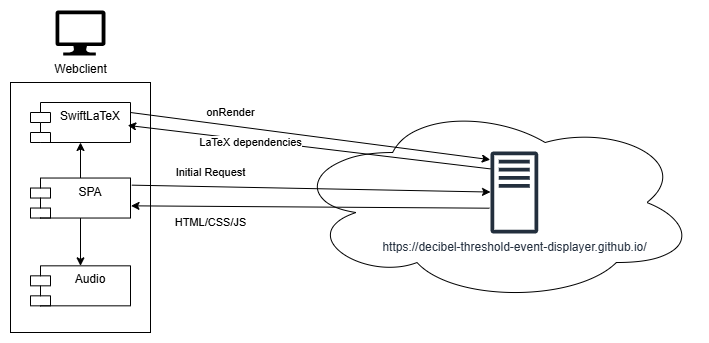
\includegraphics[width=0.8\textwidth]{../assets/high_level_architecture.png}
    \caption{Class diagram}\label{fig:high-level-architecture}
\end{figure}

\subsubsection{Data Structures and Overview}
For conveniently accessing the data contained in the wave file, we created the WaveFileWrapper class.
The wrapper is used by the home components to access the relevant data needed to create an instance of the FrameCollection class.
A FrameCollection object contains all Frame objects of the audio file and a single instance of the Frame class represent a set of samples covering a time span of 300ms.
A full overview of the data structures and how they are related to each other can be seen in~\ref{fig:class-diagram}

\begin{figure}[H]
    \centering
    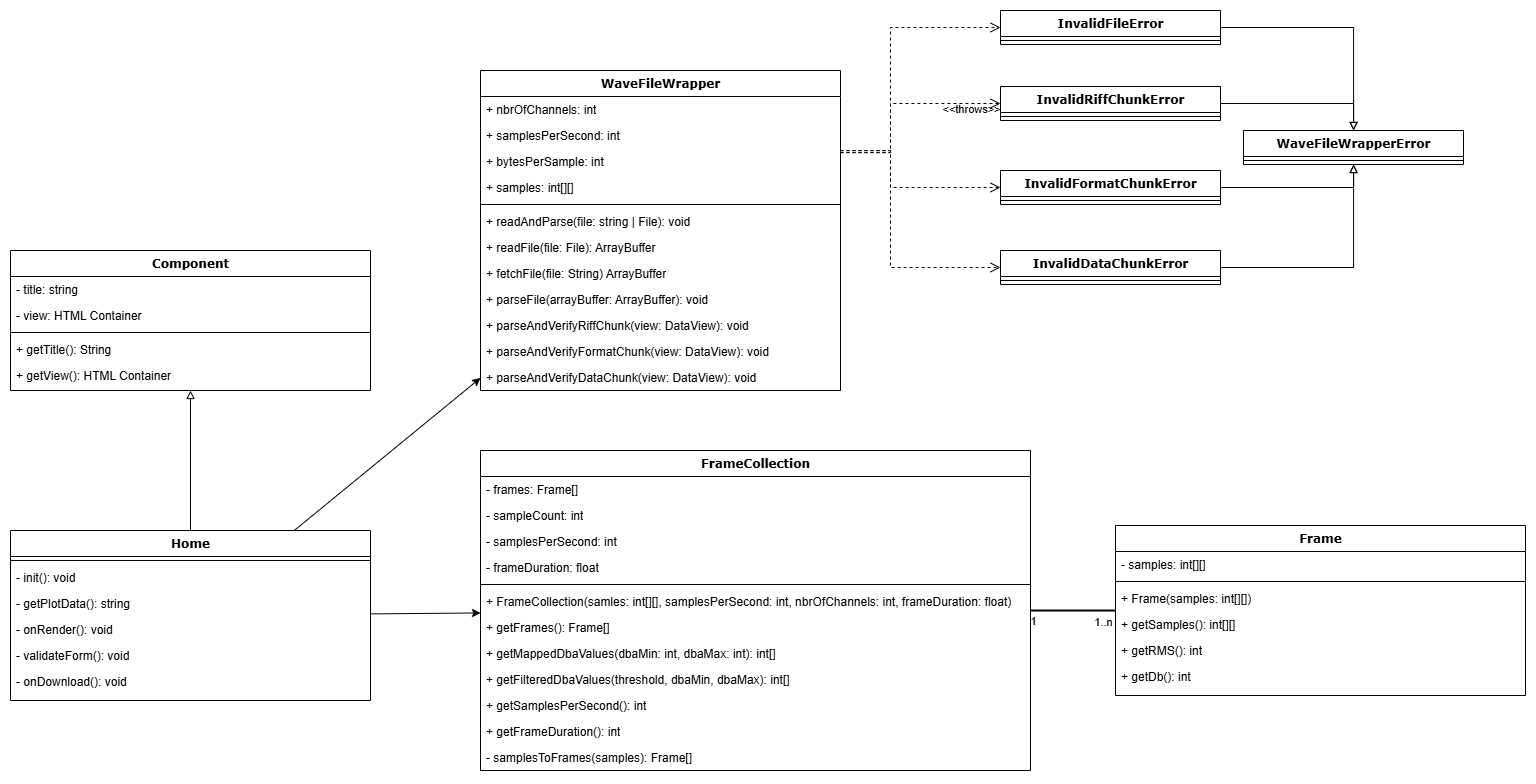
\includegraphics[width=0.8\textwidth]{../assets/class_diagram.png}
    \caption{Class diagram}\label{fig:class-diagram}
\end{figure}

\subsubsection{JavaScript Frontend (SPA)}
The frontend hosted on \href{https://decibel-threshold-event-displayer.github.io/}{Github Pages} is implemented as a single page application (SPA) following the architecture provided by the BFH in the module BTI1301 Web Programming.
In this architecture, the web server provides the index.html file as and uses JavaScript to manage the web contents (DOM updates) without changing the HTML file itself.
The project team chose to implement a small framework allowing for future expansion without rewriting the entire application.
Since the application uses SwiftLaTeX, which is run locally using WebAssembly, the SPA provides an interface for the PDF engine to its components.
The Single Page Applications Architecture is visualized in~\ref{fig:spa-architecture}

\begin{figure}[H]
    \centering
    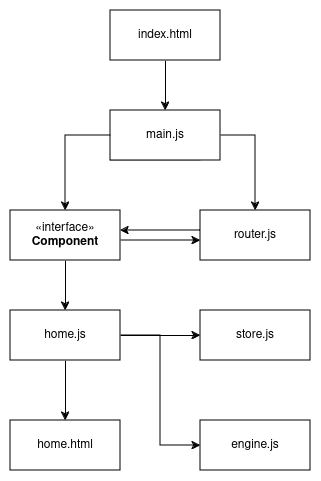
\includegraphics[width=0.4\textwidth]{../assets/spa_diagram.png}
    \caption{SPA Architecture}\label{fig:spa-architecture}
\end{figure}

In order to ensure a consistent and agreeable look, the project team has decided to use \href{https://getbootstrap.com/}{Bootstrap}, which is \href{https://github.com/twbs/bootstrap/blob/main/LICENSE}{licensed under MIT}.

We also decided to define default values for the threshold that the audio should get checked against,
for which we have orientated ourselves on the immission limits from the \href{https://www.bafu.admin.ch/bafu/de/home/themen/laerm/fachinformationen/laermbelastung/grenzwerte-fuer-laerm/belastungsgrenzwerte-fuer-laerm.html}{BAFU}.

\clearpage

\subsection{Processes}
The following diagram~\ref{fig:sequence-diagram-noise-report} gives a broad overview over the core steps involved when creating a noise report from a wave file.

\begin{figure}[H]
    \centering
    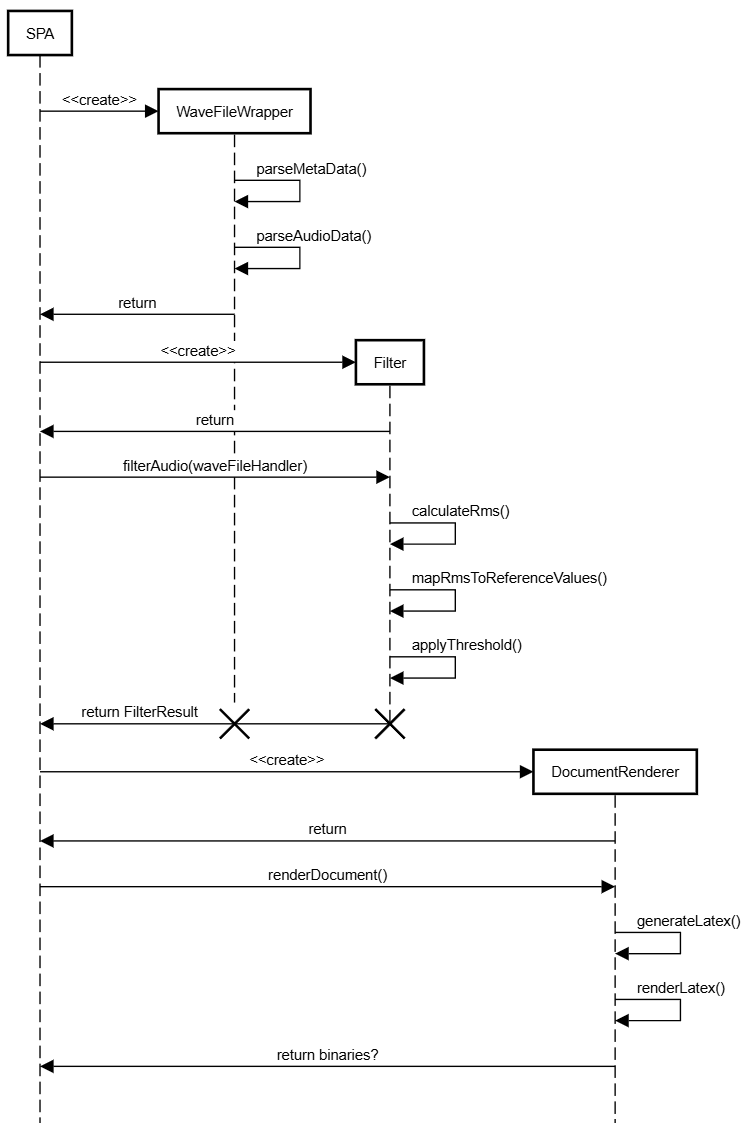
\includegraphics[width=0.9\textwidth]{../assets/sequence_diagram_from_wave_file_to_pdf.png}
    \caption{Sequence diagram of the steps involved when creating a noise report}\label{fig:sequence-diagram-noise-report}
\end{figure}

\subsubsection{Parsing the Wave File}
The WaveFileWrapper class will be responsible for reading and parsing the wave file.
Reading a file in a web context always works asynchronous, which is why there is a helper function `readAndParse` which has to be called with async/await.
The format itself is straight forward\cite{wav_file_format_wikipedia}, the only important thing is that the whole file is Little-Endian.
It starts with a 12 byte header which we use to verify that the given file is actually a wave file.
After the header comes a 24 byte chunk which contains information about the data format.
We are interested in the following fields:
\begin{itemize}
    \item AudioFormat (2 bytes): we only support PCM and IEEE Float format
    \item NbrChannels (2 bytes): is used to parse individual samples
    \item Frequency (4 bytes): number of samples per second, this is needed for filtering and summarising
    \item BitsPerSample (2 bytes): number of bits for a single sample for a single channel, is used to parse individual samples
\end{itemize}
After the format chunk can come several optional metadata chunks, which we don't need. Therefore we skip those chunks and go straight to the data chunk.
This chunk starts with a 4 byte long DataBlocID, which should always have the value `data`.
The next 4 byte represent the number of samples in the data.
After that comes the actual audio data.
To parse a single sample, we need to parse a frame.
A frame contains the data of all channels and has therefore a size of \[\frac{NbrChannels * BitsPerSample}{8}\] bytes.
Because we support 16, 24 and 32 bit integer format, as well as the IEEE float format, we have to be careful how we read the individual bytes. 
For reading the samples we use the dedicated bytes read functions like getInt16() or getFloat(32) provided by the javascript dataview object.

\subsubsection{Calculating Decibel Values}
If an audio file consists of several channels, we use the average of the channels as the value of the sample.
When we want to analyze where a certain decibel threshold has been exceeded, we must have accurate values.
People only perceive something as loud if it is loud over a longer period of time.
Short peaks are perceived less.
Therefore, when determining the effective loudness of audio, we do not use the loudness of individual samples,
but rather the average of a number of samples over a certain period of time.
Such group of samples over a certain period of time is implemented as the Frame class. The FrameCollection class represents
a list of frames for a whole audio file.
We will, as usual when working with audio, use the root-mean-square (RMS), as we are interested in the absolute amplitude values.

We implemented the calculation of the root-mean-square as the method `getRMS()` on the Frame class,
which in turn calls the rms function shown in~\ref{lst:javascript-function-rms}.

\begin{lstlisting}[caption={JavaScript RMS function},label={lst:javascript-function-rms},language=JavaScript]
/**
 * values: a list of samples, if the samples has multiple channels they need to be averaged beforehand
 */
function rms(values){
    const squared = values.map(sample => Math.pow(sample, 2));
    const sum = squared.reduce((a, b) => a + b);
    const mean = sum / values.length;
    return Math.sqrt(mean);
}
\end{lstlisting}

The calculated average then depends heavily on how long the time period is.
In practice, 300ms is usually used~\cite{timespan_for_audio_rms_calculate}.
The decibel value is calculated with the formula shown in ~\ref{lst:javascript-function-rms-to-db}, which we derived from ~\cite{decibel_wikipedia}.

\begin{lstlisting}[caption={JavaScript RMS to DB function},label={lst:javascript-function-rms-to-db},language=JavaScript]
/**
 * rms: a rms value
 */
function rmsToDb(rms) {
    return 20 * Math.log10(rms);
}
\end{lstlisting}

We implemented again a method `getDb()` on the Frame class, which computes this value.

\paragraph{Mapping RMS to absolute dB(A) values}
As mentioned in the introduction, the audio file only contains relative values.
We therefore need to map the RMS values to the number range of the reference values,
where the smallest sample is mapped to the minimal dB(A) and the largest sample is mapped to the maximal dB(A) measured.
This calculation does not work in the context of a single frame and is therefor part of the FrameCollection class. ~\ref{lst:javascript-function-db-to-dba} shows the calculation of mapping between dB and dB(A) values. 

\begin{lstlisting}[caption={JavaScript DB to DBA function},label={lst:javascript-function-db-to-dba},language=JavaScript]
/**
 * db: a frames db value from the previous calculation
 * dbMin: the minimum db value over all frames
 * dbMax: the maximum db value over all frames
 * dbaMin: the minimum dB(A) value, provided by the user
 * dbaMax: the maximum dB(A) value, provided by the user
 */
function dbToDba(db, dbMin, dbMax, dbaMin, dbaMax) {
    return (db - dbMin) * (dbaMax - dbaMin) / (dbMax - dbMin) + dbaMin;
}
\end{lstlisting}

\paragraph{Filter dB(A) values}
One of the requirements is to plot the dB(A) values which are higher than a certain threshold.
For this reason we implemented the method `getFilteredDbaValues(threshold, dbaMin, dbaMax)` which returns the final output,
which we can plot to a PDF file.

\subsubsection{LaTeX Renderer / PDF engine}\label{subsubsec:latex-renderer-pdf-engine}
As we already stated the application leverages SwiftLaTex for rendering a LaTeX template to a PDF Document, via WebAssembly.
The implementation details can be found on the following two resources:

\begin{itemize}
    \item \href{https://www.swiftlatex.com/}{SwiftLaTeX Webiste}
    \item \href{https://github.com/SwiftLaTeX/SwiftLaTeX/}{SwiftLaTeX GitHub Repository}
\end{itemize}

We integrated SwiftLaTeX into our application by downloading the~\href{https://github.com/SwiftLaTeX/SwiftLaTeX/releases/tag/v20022022}{latest release (20/02/2022)}
and unpack it to the directory `app/js/swiftlatex/lib/` and move the file `swiftlatexpdftex.js` to the parent directory `app/js/swiftlatex/`.
This way we don't have to add a dependency management tool such as npm and can we could customize the code as needed.
The application does the following steps at runtime:
\begin{enumerate}
    \item Load the LaTeX template: `app/js/swiftlatex/template.tex`
    \item Replace the placeholders in the template with the actual values (interpolate)
    \item Handover the output to SwiftLaTeX
    \item Return the resulting PDF
\end{enumerate}

\textbf{Performance improvements}
Generating the PDF file from a LaTeX document in the browser takes quite some time, as it loads all dependencies on the fly.
To speed up this process, we serve all required LaTeX files ourselves and prefetch them in parallel.
This means we have to download all LaTeX files from a public source, we are using the same source as SwiftLaTeX:
\href{https://texlive2.swiftlatex.com/}{texlive2.swiftlatex.com}

We collected all required LaTeX dependencies by modifying the SwiftLaTeX JavaScript, in such a way that during a sample
all requests pdf generation, are stored in an array, which is then printed to the console.
We put the console output in the file ``app/dependencies.json`` and created a python script under ``app/download\_dependencies.py``,
which downloads all LaTeX files to the directory ``app/dependencies/``.
We then copied the contents of ``app/dependencies.json`` to ``app/dependencies.local.json`` and made the paths relative.
Now we load this file in our main JavaScript file ``app/app.js`` and use ``Promise.all`` together with ``fetch`` to load
all dependencies into the cache of the browser.

Currently, this process involves some manual steps and could be automated in a later step.

\subsection{User Experience (UX)}\label{subsec:ux}
\subsubsection{Main Page}\label{subsubsec:main-page}
The user experience (frontend) was implemented according to the specification \ref{subsubsec:ux_prototyping} where possible.
The project team decided to use Bootstrap v5 to provide coherent look and because it is licensed under MIT. Except for the dropzone to upload files,
all components are provided in vanilla Bootstrap. Unfortunately, Bootstrap does not provide a built-in component to style the file upload as a dropzone.
The project team decided against implementing another library due to the additional upkeep required. Instead, they decided for using the file input provided by Bootstrap.
See the frontend implementation in the respective figures \ref{fig:implementation-frontend} \ref{fig:implementation-tooltip}.
\begin{figure}[H]
    \centering
    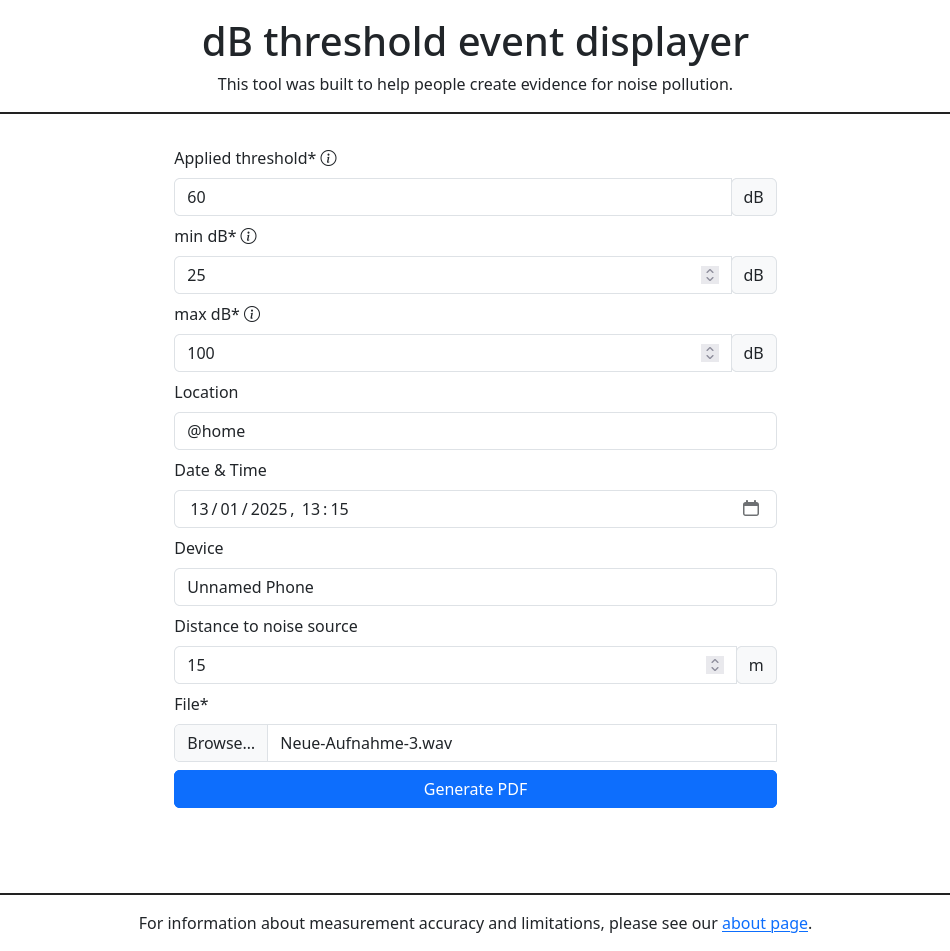
\includegraphics[width=0.75\textwidth]{../assets/implementation_form.png}
    \caption{Frontend Implementation}\label{fig:implementation-frontend}
\end{figure}
\begin{figure}[H]
    \centering
    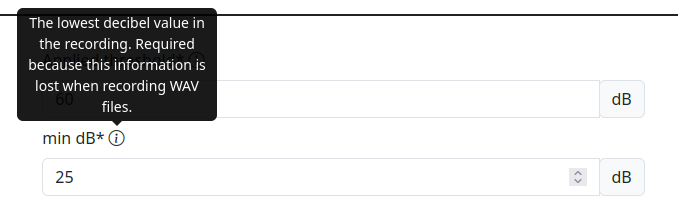
\includegraphics[width=0.5\textwidth]{../assets/implementation_tooltip.png}
    \caption{Tooltip}\label{fig:implementation-tooltip}
\end{figure}
In order to support the user when determining thresholds, the applied threshold form field is implemented as a datalist tag. This allows the user to input custom values, while
providing suggestions for pre-determined values \ref{fig:implementation-threshold}.
\begin{figure}[H]
    \centering
    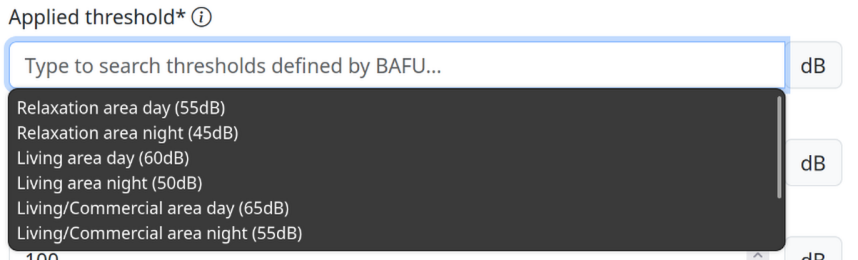
\includegraphics[width=0.5\textwidth]{../assets/implementation_threshold.png}
    \caption{Default Thresholds}\label{fig:implementation-threshold}
\end{figure}
Another departure from the specification was the addition of a separate about page \ref{subsubsec:about-page}. Since it was easy to implement,
the project team has also decided to add a preview for the rendered document alongside the download button. This also improves feedback because it allows the user to
check what the file looks like before saving, letting them check for typos and other issues \ref{fig:implementation-preview}.
\begin{figure}[H]
    \centering
    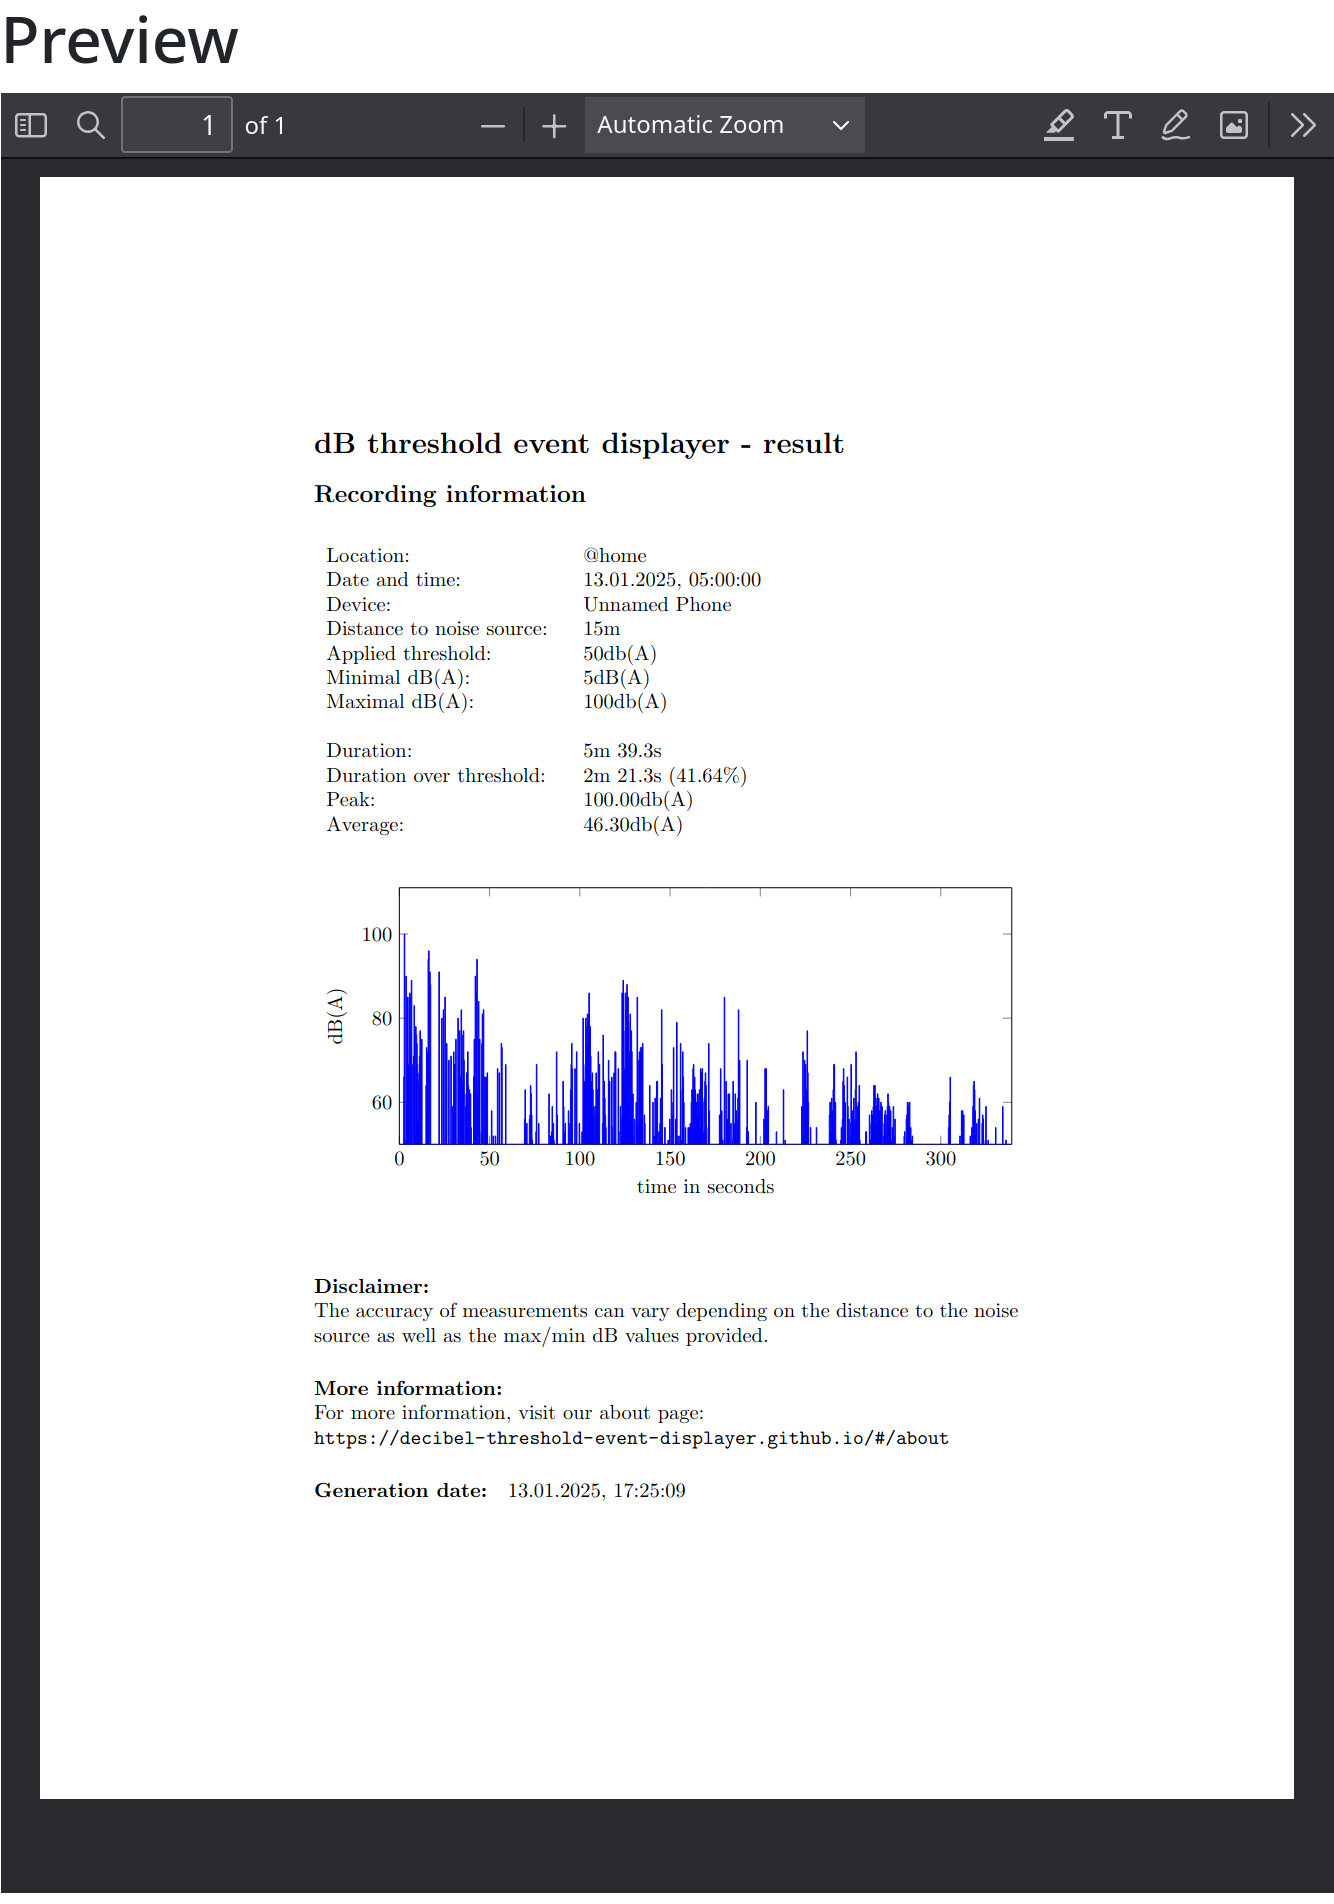
\includegraphics[width=0.75\textwidth]{../assets/implementation_preview.png}
    \caption{Report Preview}\label{fig:implementation-preview}
\end{figure}
To provide additional feedback and ensure consistent results, the project team has also implemented
validations for the important input fields \ref{fig:implementation-validation}.
\begin{figure}[H]
    \centering
    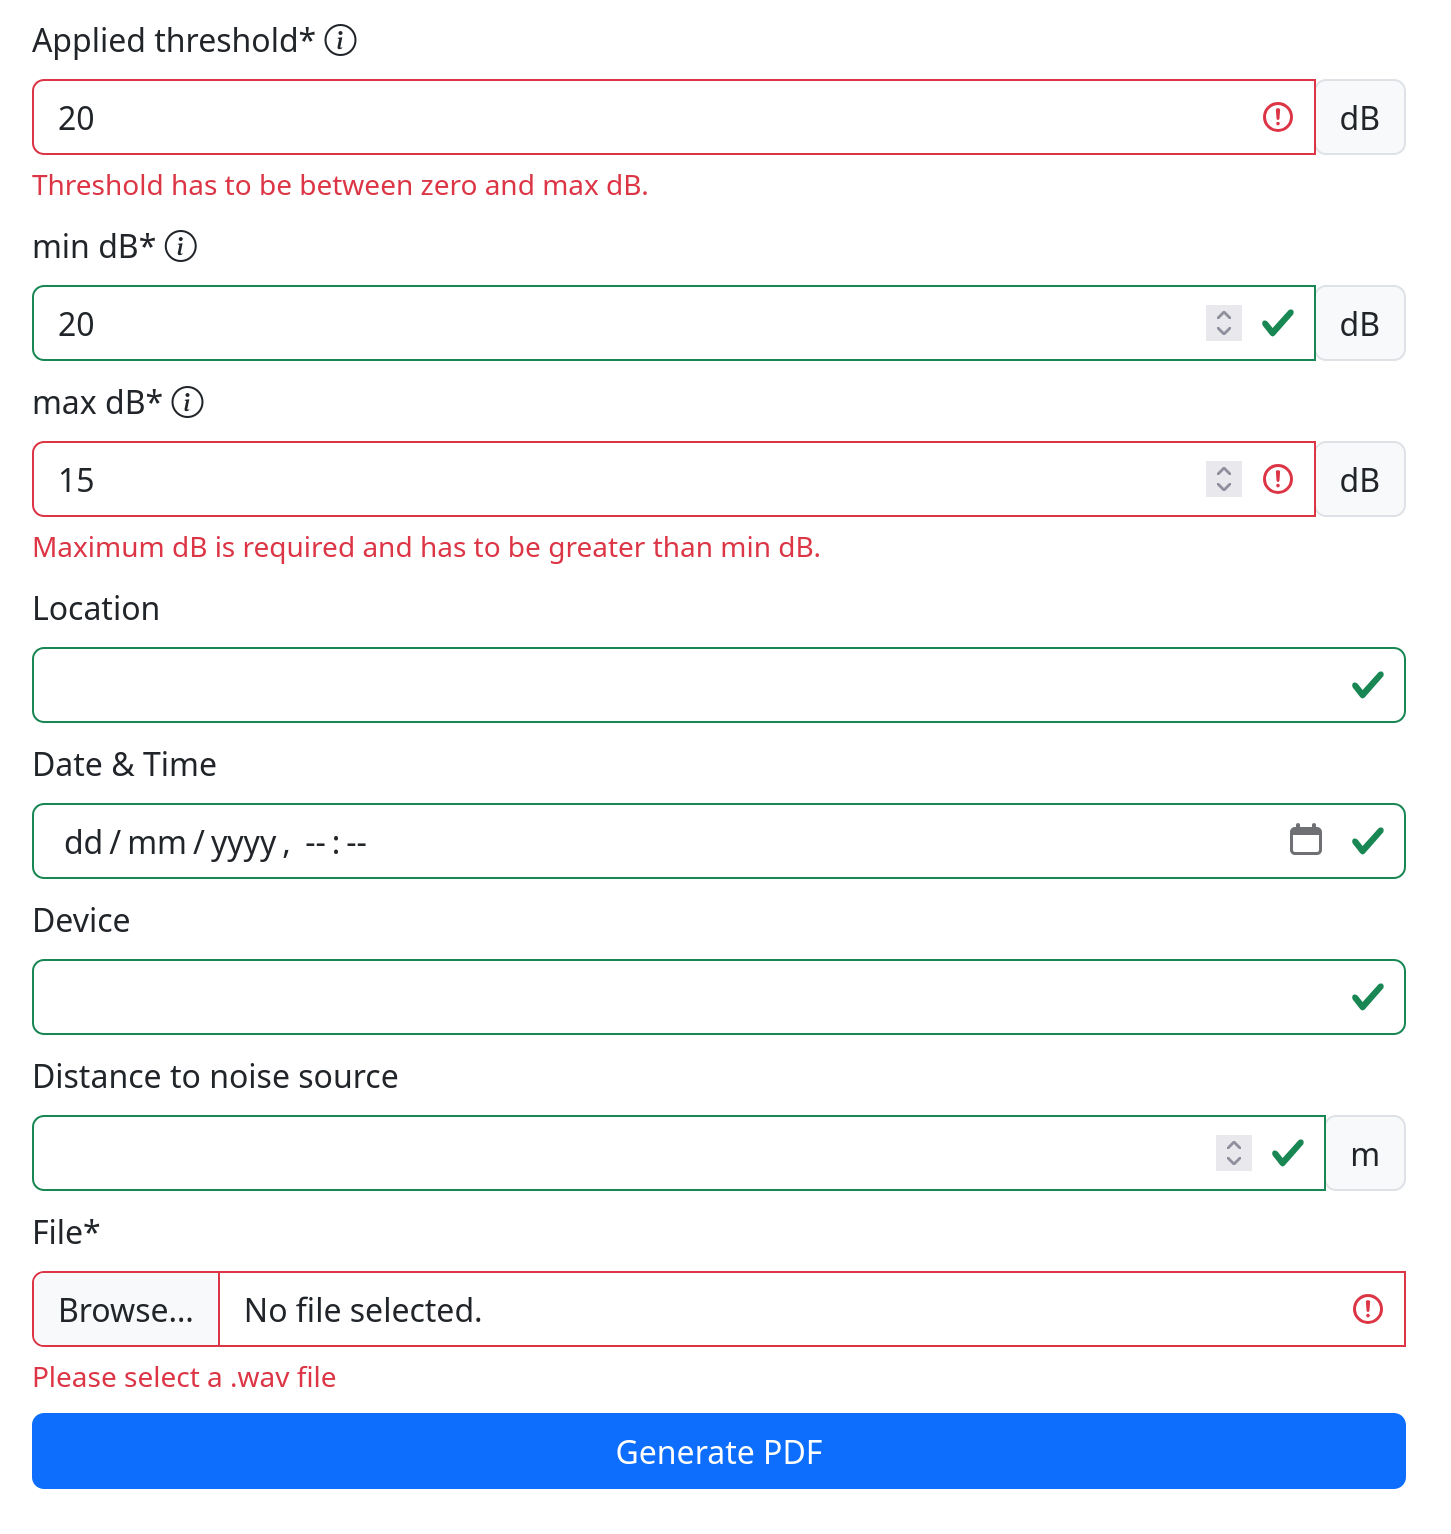
\includegraphics[width=0.75\textwidth]{../assets/implementation_validation.png}
    \caption{Form Validation}\label{fig:implementation-validation}
\end{figure}

\subsubsection{About Page}\label{subsubsec:about-page}
To provide users with additional information about the application's implementation, privacy concerns, calculation details, as well as an impressum, the project team implemented
a separate about page. There is also a link to the GitHub repository, as well as a disclaimer about the accuracy of the results. See \ref{fig:implementation-about-page} for an excerpt of the implementation.
\begin{figure}[H]
    \centering
    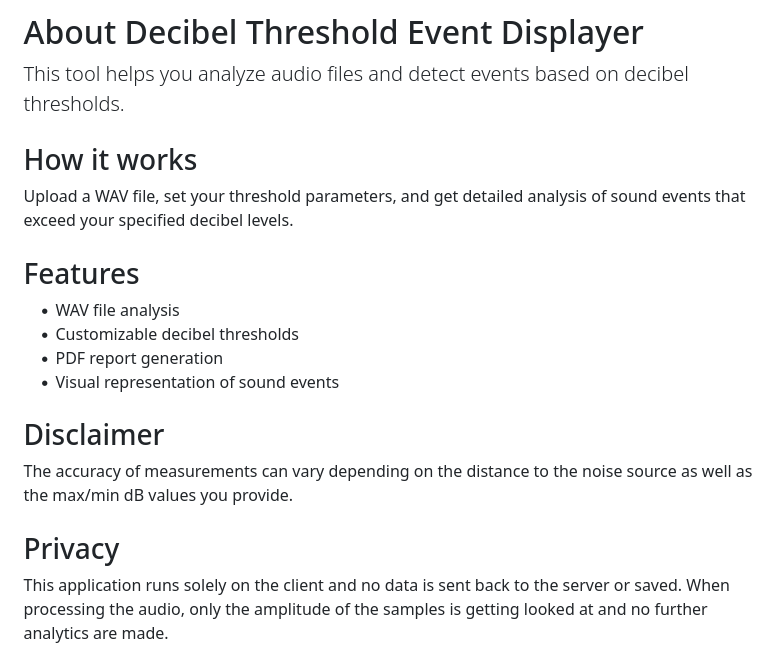
\includegraphics[width=0.75\textwidth]{../assets/implementation_about_page.png}
    \caption{About Page excerpt}\label{fig:implementation-about-page}
\end{figure}

\subsection{Testing}\label{subsec:testing}
Because we don't use any Frontend Framework and instead build our own SPA, we don't have a testing framework to use.
We therefore decided to build our own rudimentary testing framework.
It consists out of 4 assert functions, a test runner and a html page for displaying the results.
There is no automatic mechanism running the tests after every commit, the tests have to be run manually.

As we are developing an application for analyzing a wave file, nearly every tests first step is to create a WaveFileWrapper object for further use.
Because the reading and parsing of the file works asynchronous, the test suit has also to be asynchronous.
We decided to use the async/wait approach instead of using promises because promises are more difficult to debug, which is not suitable for a test framework.
The following diagram~\ref{fig:overview-test-framework} shows the internal structure of the test framework.

\begin{figure}[H]
    \centering
    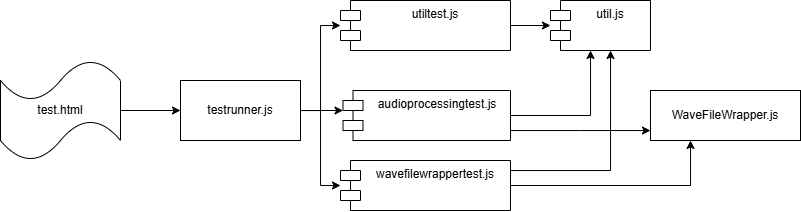
\includegraphics[width=0.8\textwidth]{../assets/overview_test_framework.png}
    \caption{Overview test framework}\label{fig:overview-test-framework}
\end{figure}

\subsubsection{Assert functions}
For implementing tests there are 5 assert functions contained in the util module which can be used:

\begin{itemize}
    \item assertThrows: verifies that a certain exception is thrown
    \item assertNotThrows: verifies that no exception is thrown
    \item assertEquals: verifies that something is equal to a given value
    \item assertNotEquals: verifies that something is not equal to a given value
    \item assertGreaterThen: verifies that a number is greater the other
\end{itemize}

If the assertion of a function fails, it throws an exception with some information on why the test failed.
The assertEquals and assertNotEquals function work with any kind of object.
They first stringify both objects to a json format and then compare the json.
It is certainly not the most efficient method, but it works for all cases.
The assertThrows and assertNotThrows both take in a function which will be called in the assert function itself and verified that it throws or not throws an exception.
The assertGreaterThen can also take in two arguments from any type, as JavaScript allows such comparisons.
With those functions we were able to implement all our tests.
To make sure that the assert functions work, we implemented also tests for them.
Those test obviously don't use the assert functions and rather have some hard coded tests created for them.
Those tests can be found in the utiltest module.

\subsubsection{Creating tests}
To create tests, one has to create a JavaScript file containing its tests under `app/js/test/`.
All functions that are being exported by the given JavaScript file are considered to be tests and will be executed by the test runner.
If a function throws an exception, it is assumed that the test failed.
If no exception is thrown, the test passes.
We tried to keep the manual work for adding tests minimal, but some manual work is still necessary.
To add a new test module, the module has to be imported into the test runner file as shown in~\ref{lst:javascript-test-framework-importing-module-with-tests}.
After that, a new call to the function runTestGroup can be added as it's shown in~\ref{lst:javascript-test-framework-adding-a-method-call-to-run-a-test-module}, which will then add the test.
Take a look at the existing tests as a reference.

\begin{lstlisting}[caption={Importing a module with tests},label={lst:javascript-test-framework-importing-module-with-tests},language=JavaScript]
import * as waveFileWrapperTest from './wavefilewrappertest.js';
import * as audioProcessingTest from './audioprocessingtest.js';
import * as utilTest from './utiltest.js';
\end{lstlisting}

\begin{lstlisting}[caption={Adding a method call to run a test module},label={lst:javascript-test-framework-adding-a-method-call-to-run-a-test-module},language=JavaScript]
/**
 * Runs all test modules in sequence.
 */
function runTests() {
    runTestModule(utilTest, "Util");
    runTestModule(waveFileWrapperTest, "Wave File Wrapper");
    runTestModule(audioProcessingTest, "Audio Processing");
}
\end{lstlisting}

\subsubsection{Test runner}
The test runner is responsible for running the tests.
It runs every test module in sequence and summarises its results.
For each module a table in the result page is created which contains the test names, result and in the case of a failed test a message why it failed.
The tests are run when the dedicated button in the frontend is pressed.
The test runner always runs every test of every test module.
There is currently no function to run individual modules or tests.
The test runner also has a function to just test the WaveFileWrapper.
It creates such a WaveFileWrapper object from the file specified on the result page and displays the values of its properties.

\subsubsection{HTML page}
The fronted page of the test framework is used to start the tests and view the results.
It is additionally used to create a WaveFileWrapper object and view the properties of it.
The test page is accessible under \href{https://decibel-threshold-event-displayer.github.io/js/test/test.html}{/js/test/test.html}.
To run the test page on the dev server on localhost, see chapter~\ref{subsubsec:deployment-setup}.

The screenshot~\ref{fig:create-a-wavefilewrapper-object} shows how the test framework validated an uploaded *.wav file.
\begin{figure}[H]
    \centering
    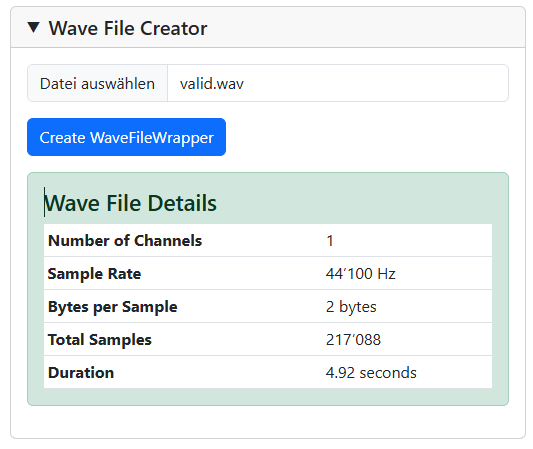
\includegraphics[width=0.8\textwidth]{../assets/wavefilecreator.png}
    \caption{Create a WaveFileWrapper object and view its properties}\label{fig:create-a-wavefilewrapper-object}
\end{figure}

On screenshot~\ref{fig:test-results} we can see the test results after running the test runner.
\begin{figure}[H]
    \centering
    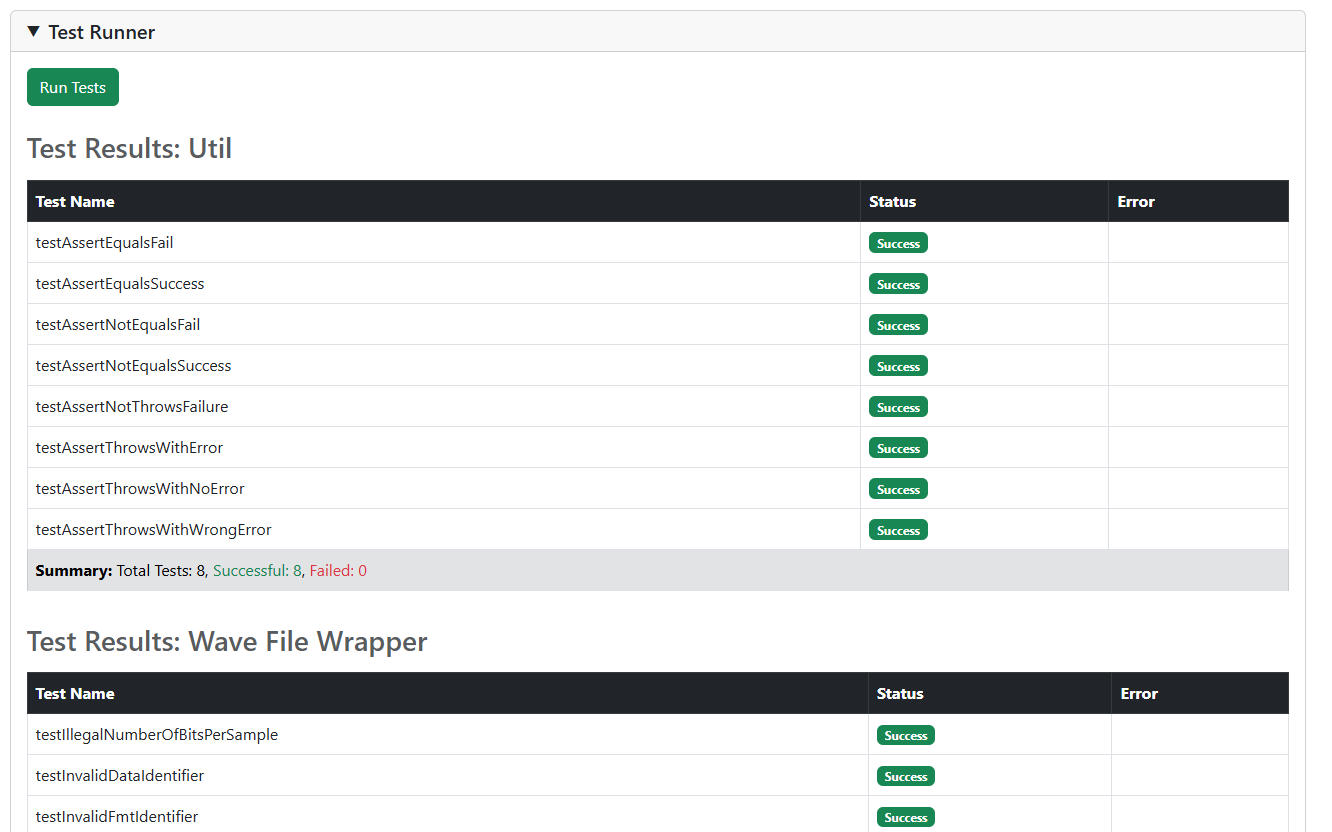
\includegraphics[width=0.8\textwidth]{../assets/test_results.png}
    \caption{Test results}\label{fig:test-results}
\end{figure}
